\documentclass[12pt]{article}

% This first part of the file is called the PREAMBLE. It includes
% customizations and command definitions. The preamble is everything
% between \documentclass and \begin{document}.

\usepackage[margin=1in]{geometry}  % set the margins to 1in on all sides
\usepackage{graphicx}              % to include figures
\usepackage{amsmath}               % great math stuff
\usepackage{amsfonts}              % for blackboard bold, etc
\usepackage{amsthm}                % better theorem environments
\usepackage{listings}
\usepackage{multirow}
\usepackage{hyperref}
\usepackage{parskip}
\usepackage{color}
% various theorems, numbered by section
\newcommand{\red}[1]{\textsf{\textbf{\textcolor{red}{[#1]}}}}
\begin{document}


\title{NxRepair: Error Correction in De Novo Sequence Assembly Using Nextera Mate Pairs}

\author{Rebecca R. Murphy, Jared O'Connell, Anthony J. Cox and Ole Schulz-Trieglaff \\ 
Illumina Cambridge, Chesterford Research Park, Essex, CB10 1XL}

\maketitle

\begin{abstract}
  Supplementary Information for the paper NxRepair: Error Correction in De Novo Sequence Assembly Using Nextera Mate Pairs 
\end{abstract}

\section{Prior Work}
Error correction in de novo assemblies is a well-studied problem. Recent work, such as the Assemblathon~\cite{Bradnam2013} and GAGE~\cite{Salzberg2012} collaborations compare the quality of assemblies prepared by various assemblers. A Bayesian method of assembly quality evaluation also exists~\cite{Ghodsi2013}. Several recent papers have developed error identification and correction methods. The A5 Assembly Pipeline~\cite{Coil2014} includes an error detection and rescaffolding step and two new tools, REAPR~\cite{Hunt2013} and ALE~\cite{Clark2013} use read pair data to identify misassemblies. A similar tool is currently under development at the Broad Institute~\cite{pilon2014}. NxRepair is complementary to these tools, as it specifically uses Nextera mate-pair information to find the largest and most serious misassemblies: REAPR and A5-MiSeq do not use mate-pair information and ALE is unfortunately no longer in active development.

\section{Supplementary Methods}
\subsection{Data}
Nine bacterial genomes were prepared according to the Nextera Mate Pair protocol and sequenced in a single MiSeq run using $2 \times 151$ bp reads. The genomes sequenced are shown in Table~\ref{data-description}. Reads were trimmed using the MiSeq inbuilt trimmer. The untrimmed reads are available from BaseSpace via \url{https://basespace.illumina.com/s/TXv32Ve6wTl9} (free registration required). Note that only these Nextera mate pair libraries were used. No additional single end or paired end libraries were required.   

\begin{table}[h]
  \centering
\resizebox{\textwidth}{!}{
  \begin{tabular}{ll}
    \hline
    \textbf{Abbreviation:}             &    Bcer \\
    \textbf{Bacteria:}                 &    \emph{Bacillus cereus ATCC 10987} \\
    \textbf{Accession ID:}  &  NC\_003909, NC\_005707 \\ 
    \textbf{NCBI FTP:}                 &    \url{ftp.ncbi.nih.gov/genomes/Bacteria/Bacillus\_cereus\_ATCC\_10987\_uid57673/} \\
    \hline
    \textbf{Abbreviation:}             &    EcDH \\ 
    \textbf{Bacteria:}                 &    \emph{Escherichia coli str. K-12 substr. DH10B}\\ 
    \textbf{Accession ID:}              &    NC\_010473 \\ 
    \textbf{NCBI FTP:}     &    \url{ftp.ncbi.nih.gov/genomes/Bacteria/Escherichia\_coli\_K\_12\_substr\_\_DH10B\_uid58979/}\\
    \hline
    \textbf{Abbreviation:}             &   EcMG \\
    \textbf{Bacteria:}                 & \emph{Escherichia coli str. K-12 substr. MG1655}\\
    \textbf{Accession ID:}            & NC\_000913    \\ 
    \textbf{NCBI FTP:}       & \url{ftp.ncbi.nih.gov/genomes/Bacteria/Escherichia\_coli\_K\_12\_substr\_\_MG1655\_uid57779/}\\
    \hline
    \textbf{Abbreviation:}             &   list\\ 
    \textbf{Bacteria:}                 &\emph{Listeria monocytogenes}\\  
\textbf{Accession ID:}              & NC\_003210 \\ 
\textbf{NCBI FTP:}     & \url{ftp.ncbi.nih.gov/genomes/Bacteria/Listeria\_monocytogenes\_EGD\_e\_uid61583/}\\
\hline
\textbf{Abbreviation:}             &  meio \\ 
\textbf{Bacteria:}                 &\emph{Meiothermus ruber DSM 1279}\\ 
\textbf{Accession ID:}             &NC\_013946 \\ 
\textbf{NCBI FTP:}      & \url{ftp.ncbi.nih.gov/genomes/Bacteria/Meiothermus\_ruber\_DSM\_1279\_uid46661/}\\
   \hline
\textbf{Abbreviation:}             &  ped \\
\textbf{Bacteria:}                 &\emph{Pedobacter heparinus DSM 2366}\\
\textbf{Accession ID:}                 & NC\_013061 \\ 
\textbf{NCBI FTP:}  & \url{ftp.ncbi.nih.gov/genomes/Bacteria/Pedobacter\_heparinus\_DSM\_2366\_uid59111/}\\
   \hline
\textbf{Abbreviation:}             &   pneu \\
\textbf{Bacteria:}                 & \emph{Klebsiella pneumoniae subsp. pneumoniae MGH 78578}  \\
\textbf{Accession ID:}              & NC\_009648, NC\_009649, NC\_009650, NC\_009651, NC\_009652, NC\_009653 \\ 
\textbf{NCBI FTP:}     & \url{ftp.ncbi.nih.gov/genomes/Bacteria/Klebsiella\_pneumoniae\_MGH\_78578\_uid57619/}\\
   \hline
\textbf{Abbreviation:}             &  rhod \\ 
\textbf{Bacteria:}                 &\emph{Rhodobacter sphaeroides 2.4.1}\\ 
\textbf{Accession ID:}                 &NC\_007488, NC\_007489, NC\_007490, NC\_007493, NC\_007494, NC\_009007, NC\_009008\\ 
\textbf{NCBI FTP:}  & \url{ftp.ncbi.nih.gov/genomes/Bacteria/Rhodobacter\_sphaeroides\_2\_4\_1\_uid57653/}\\ 
   \hline
\textbf{Abbreviation:}             &  TB \\
\textbf{Bacteria:}                 & \emph{Mycobacterium tuberculosis H37Ra}\\ 
\textbf{Accession ID:}               &NC\_009525 \\ 
\textbf{NCBI FTP:}    & \url{ftp.ncbi.nih.gov/genomes/Bacteria/Mycobacterium\_tuberculosis\_H37Ra\_uid58853/}\\ 
   \hline
  \end{tabular}
}
  \caption{Summary of bacteria analysed and the relevant NCBI information on their reference genomes. There were two repeats of each strain. All 18 samples were prepared with the Nextera Mate Pair protocol and sequenced in a single MiSeq run using $2 \times 151$ bp reads. The untrimmed reads we used as input to NxTrim (3.9Gbp in all) are available from BaseSpace via \url{https://basespace.illumina.com/s/TXv32Ve6wTl9} (free registration required).\label{data-description}}
\end{table}

\subsection{Workflow Pipeline}
De novo assemblies were prepared using the SPAdes Assembler, version 3.1.1~\cite{Bankevich2012}:

\texttt{spades.py -k 21,33,55,77 -t 4 --careful --hqmp1-12 bacteria.fastq.gz  --hqmp1-fr -o assembly}

The initial assembly quality was evaluated using QUAST~\cite{gurevich2013} to aligning the de novo assembly to a reference genome:

\texttt{python quast.py -o results\_sample -t 16   -R ref/referenece.fna sample\_new.fasta }

Following assembly of the remaining seven genomes, the mate-pair reads were aligned back to the de novo assembly using BWA-MEM~\cite{li2013}. A sorted bam file of the resulting alignment was then prepared using SAMtools~\cite{li2009}: 

\texttt{bwa index sample/scaffolds.fasta}

\texttt{bwa mem sample/scaffolds.fasta -p bacteria.fastq.gz | samtools view -bS - |  samtools sort - sample}

\texttt{samtools index sample.bam}

We identified misassemblies using NxRepair as follows:

\texttt{python nxrepair.py sample.bam   sample/scaffolds.fasta sample\_scores.csv  sample\_new.fasta -img\_name sample\_new}


The default parameters used and their meanings are shown in Table~\ref{tab:parameters}. These have been optimised for Illumina Nextera mate-pair libraries with a mean insert size of approximately 3 Kb. For mate-pair libraries with a much larger (smaller) insert size, the maxinsert and trim parameters may need to be increased (decreased).

\begin{table}
\begin{center}
\begin{tabular}{|c|c|p{8cm}|}
    \hline
    Parameter & Default Value & Meaning \\ \hline
    imgname & None & Prefix under which to save plots. \\
    maxinsert & 30000 &  Maximum insert size, below which a read pair is included in calculating population statistics.\\
    minmapq & 40 & Minimum MapQ value, above which a read pair is included in calculating population statistics.\\
    minsize & 10000 & Minimum contig size to analyse.\\ 
    prior & 0.01 & Prior probablility that the insert size is anomalous.\\
    stepsize & 1000 & Step-size in bases to traverse contigs.\\
    trim & 4000 & Number of bases to trim from each side of an identified misassembly.\\
    T & -4.0 & Threshold in Z score (number of standard deviations from the mean) below which a misassembly is called.\\
    window & 200 & Window size across which bridging mate pairs are evaluated.\\ \hline
\end{tabular}
\end{center}
\caption{NxRepair Parameters \label{tab:parameters}}
\end{table}

Finally we used QUAST~\cite{gurevich2013} to evaluate the assembly quality following NxRepair by aligning the de novo assembly to a reference genome as described above.

\section{Implementation}
\subsection{Global Assembly Parameters}
NxRepair identifies misassemblies based on the insert size distribution of mate pairs aligned to the de novo assembly. The first step is calculation of the global mate pair insert size distribution. For calculation of population statistics, mate pairs that align to different contigs from each other are excluded, as are mate pairs with an incorrect strand or pairing orientation, pairs whose mapping quality falls below a user specified threshold, and pairs whose insert size exceed 30 Kb (approximately 10 times the mean insert size). The global mean $\hat{\mu}$ and median absolute deviation $\text{MAD}$ were calculated across all contigs in the assembly as:

\begin{equation}
\hat{\mu} = \frac{\sum_{i=1}^N Y_i}{N} \qquad \text{MAD} = \text{median}_i(|Y_i - \text{median}_j(Y_j)|)
\label{eq:global}
\end{equation}

where $Y_l$ is the insert size of the $i$th of $N$ reads with correct pairing behaviour. These were then used as the parameters of the null distribution, as described in the main paper. The median absolute deviation was used in place of the standard deviation, as it is more robust to outlier insert sizes.

\subsection{Interval Tree Construction}
To facilitate rapid lookup of mate pair properties, we construct an interval tree~\cite{cormen2009} for each contig in the de novo assembly. An interval tree is a datastructure that facilitates $O(\text{log} n + m)$ lookup of intervals that span a given point or interval, for $n$ total entries and $m$ spanning entries. The interval tree contains the start and end positions of each mate pair aligned to that contig, as well as an flag variable indicating whether that mate pair had correct strand and pairing orientation. Mate pairs where the two pairs aligned to different contigs were excluded,  This allows NxRepair to rapidy query positions across a contig to discover the insert size distribution at the queried position.  

\subsection{Assembly Support and Z-Score Calculation}
To calculate the degree of support for the assembly at each site across a contig, NxRepair retrieves all mate pairs spanning a window of size `window' at position $i$ on the contig. As described in the main paper, we define a latent indicator variable $X_i\in\{0,1\}$ for each pair of reads, $l$, which takes the value $1$ if the insert size came from our null distribution, and $0$ otherwise. Within each window queried, the probability that each retrieved read, $r_i$ is drawn from the null distribution is given by:

\begin{eqnarray} P(X_i=x|Y_i)& =& \frac{P(X_i=x)(Y_i|X_i=x)}{\sum_{k=0}^1P(X_i=k)(Y_i|X_i=k)}\\
  & =& \frac{\pi_x(Y_i|X_i=x)}{\sum_{k=0}^1 \pi_k(Y_i|X_i=k)}
\label{eq:posterior}  
\end{eqnarray}

where $\pi_x$ is the user defined prior probability of class $x$ and $\pi_1 + \pi_0 = 1$. The default value of $\pi_0$ is 0.01 (see table~\ref{tab:parameters}), meaning that in the absence of any insert size information, 99 \% of read pairs are from the null distribution.  

Within each window, the total support for a correct assembly at position $l$ can be calculated as:

\begin{equation}
D_l = \sum_{i=1}^N P(Z_i=1|Y_i)\cdot C_i
\end{equation}

where $C_i$ is an indicator variable, reporting pairing orientation:

\begin{equation}
    C_i=
    \begin{cases}
      1, & \text{if}\ \text{mate pairs have correct orientation and strand alignment} \\
      0, & \text{otherwise}
    \end{cases}
  \label{eq:C}
  \end{equation}

Within each contig, the contig assembly support mean $\hat{\mu}_D$ and variance $s_D$ are calculated from all reads aligning to the contig,
\begin{equation}
\hat{\mu}_D = \frac{\sum_{l=1}^N D_l}{N} \qquad s_D = \frac{\sum_{l=1}^N \sqrt{(D_l - \hat{\mu})^2}}{N}
\label{eq:contigD}
\end{equation}

Using these values, the Z-score $z_l$ within each queried interval is calculated as: 

\begin{equation}
z_l = \frac{D_l - \hat{\mu}_D}{s_D}
%\hat{\mu} = \frac{\sum_l^N D_l}{N} \qquad \s = \frac{\sum_l^N \sqrt{(D_l - \hat{\mu})^2}}{N}
\label{eq:zscore}
\end{equation}

A misassembly is identified if $z_l < T$ for a user-defined threshold $T$ (default value -4). This threshold describes the number of standard deviations below the mean assembly support that is required to identify an anomaly. The default value of -4 will flag only positions whose assembly support is less than four standard deviations below the mean level of support. As the parameters of the distribution are derived from the properties of the assembly, this is robust to variation in coverage, contig size and other assembly properties.

\subsection{Misassembly Location and Contig Breaking}
To improve the quality of the de novo assembly, a contig is broken into two separate pieces at the site of a misassembly and the broken ends of the two new contigs trimmed by a user defined length (default 4 Kb) to remove the misassembled region. To prevent excessive clipping, misassemblies separated by less than the trimming distance are grouped together, the contig is broken at the start and end of the misassembled region and the misassembled section is discarded. Low-scoring regions within the trimming distance of the ends of contigs are not considered misassemblies, as the high proportion of mate pairs aligning here whose mate maps to a different contig reduces the number of pairs under consideration and hence lowers the observed Z-score.   

\subsection{Evaluation}
To evaluate the performance of NxRepair, we prepared Receiver Operating Curves (ROCs) for each bacterial genome, evaluated at a range of different thresholds. As misassemblies are identified as point errors, but our NxRepair method identifies the region spanned by a misassembly, we needed a method to correctly compare the sites of true misassemblies with those identified by NxRepair. To make this comparison, we divided each contig of the assembly into short stretches of 1 Kb length. We then prepared an array, $A_{Nx}$ of size $\frac{L}{1000}$ for contig length $L$, corresponding to misassemblies identified by NxRepair. $A_{Nx}$ was filled as follows:

%\begin{equation}
%    A_T=
%    \begin{cases}
%      1, & \text{if}\ \text{stretch $i$ contains a true misassembly} \\
%      0, & \text{otherwise}
%    \end{cases}
%  \label{eq:true}
%\end{equation} 

\begin{equation}
    A_{Nx}=
    \begin{cases}
      1, & \text{if}\ \text{NxRepair identified a misassembly in stretch $i$} \\
      0, & \text{otherwise}
    \end{cases}
  \label{eq:found}
\end{equation}

To prepare the ROCs each position $i$ in $A_{Nx}$ was labeled as true positive (TP) if $A_{Nx}[i] = 1$ and a true misassembly fell within it, true negative (TN) if $A_{Nx}[i] = 0$ and no true misassembly occurred within the interval, false positive (FP) if $A_{Nx}[i] = 1$ but no true misassembly had occurred, or false negative (FN) if $A_{Nx}[i] = 0$ but the interval contained a true misassembly. The true positive rate (TPR) false positive rate (FPR) were then calculated as follows:

\begin{equation}
\text{TPR} = \frac{\text{TP}}{\text{TP} + \text{FN}} \qquad \text{FPR} = \frac{\text{FP}}{\text{FP} + \text{TN}}
\label{eq:tpr}
\end{equation} 

The ROC plots are shown in Supp. Figure~\ref{fig:ROCs}.

\begin{figure}
\centerline{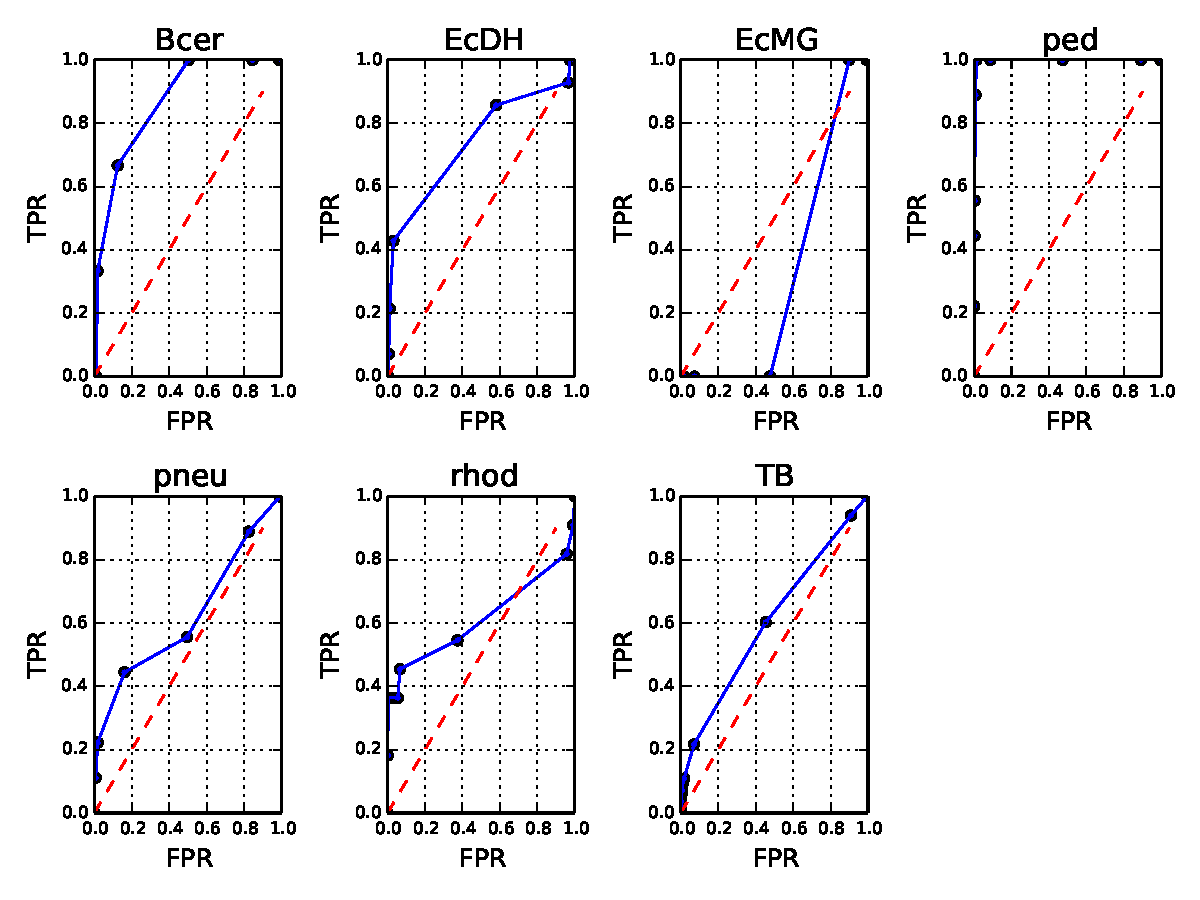
\includegraphics[width=0.8\textwidth]{allROC_extensive.pdf}}
\caption{ROC plots for each of the seven genomes evaluated here.\label{fig:ROCs}}
\end{figure}

Finally, we plotted the NGA50 value as calculated by QUAST against the NA50, before and after NxRepair correction, to demonstrate that we have not reduced the assembly quality. This is shown in Supp. Figure~\ref{fig:NGA50}. We note that in the case of the TB genome, the NGA50 was reduced by NxRepair correction. Manual inspection of the correction sites revealed that one of the misassemblies reported by nxrepair was a join between two contigs which consisted of a gap of over 2 Kb bridged by very few mate pairs. This join is reported as correct by Quast, but has only very little support from the read data.

\begin{figure}
\centerline{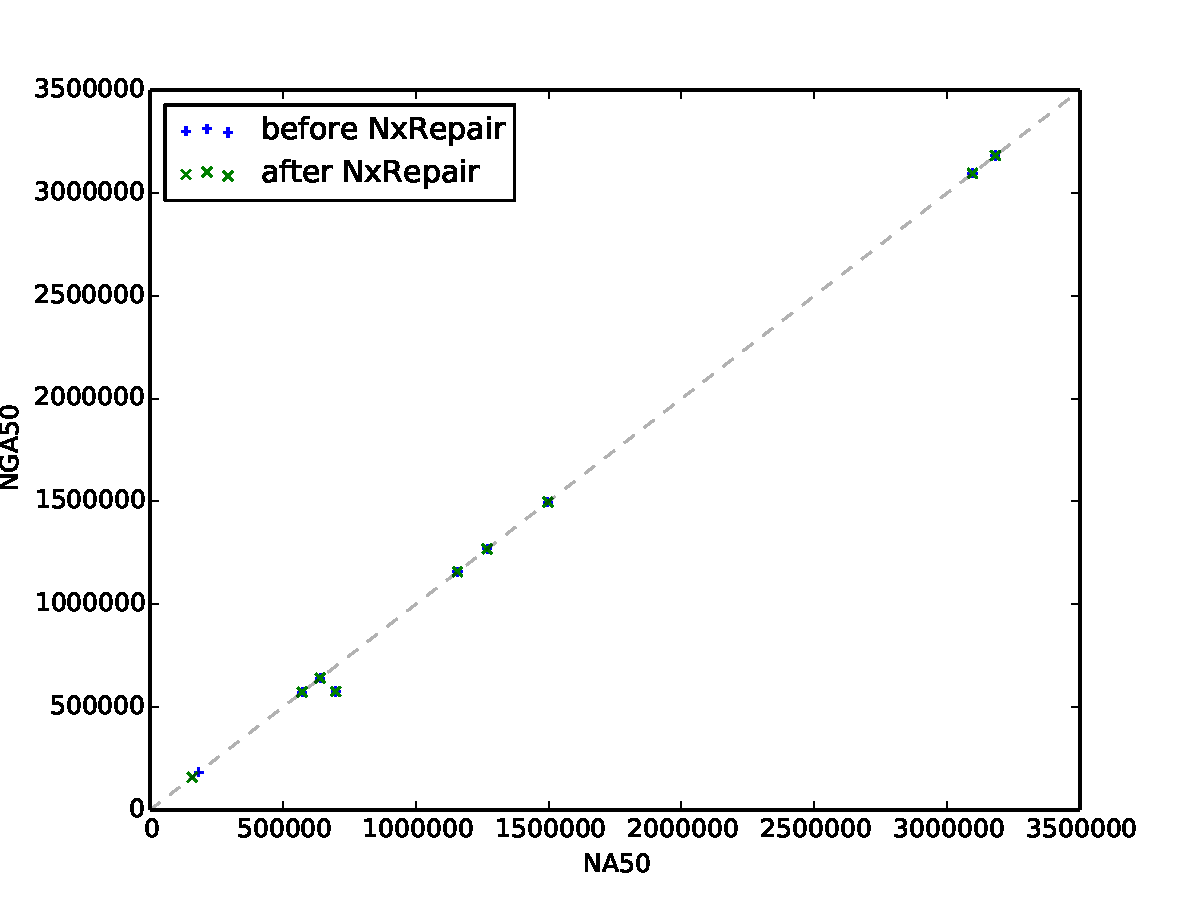
\includegraphics[width=0.8\textwidth]{ng50.pdf}}
\caption{Plot of NGA50 vs NA50 for each genome before and after NxRepair correction.\label{fig:NGA50}}
\end{figure}

\section{Performance}
We evaluated the runtime and peak memory usage of NxRepair on each of the nine genomes analysed. The results are shown in table~\ref{tab:performance}. Performance analysis was performed on a single core with GB RAM available. Runtime analysis was performed using the python cProfile module. The memoryprofiler python module was used to analyse memory usage. The most memory and compuationally intensive part of the NxRepair analysis is construction of the interval trees. The size of each interval tree constructed is dependent on the contig size. Consequently, we expect both runtime and memory usage to scale with the size of the largest contig. 

\begin{table}
\begin{center}
\begin{tabular}{|c|c|c|}
    \hline
    Bacterium & Total Time (s) & Memory Usage (MiB) \\ \hline
    Bcer & 78 & 271 \\
    EcDH & 123 & 444 \\
    EcMG & 70 & 260 \\
    list & 97 & 383 \\
    meio & 259 & 565 \\
    ped & 123 & 417 \\
    pneu & 59 & 227 \\
    rhod & 190 & 463 \\
    TB & 155 & 411 \\ 
    \hline
\end{tabular}
\end{center}
\caption{NxRepair performance analysis. \label{tab:performance}}
\end{table}

\clearpage

\section{Availibility and Dependencies}
NxRepair is available for free anonymous download from the Python Package Index (PyPI) here: \url{:https://pypi.python.org/pypi/nxrepair}.
The source code, written in python is hosted on GitHub: \url{https://github.com/rebeccaroisin/nxrepair}.
A full tutorial and API can be found on ReadTheDocs: \url{http://nxrepair.readthedocs.org/en/latest/}.

NxRepair makes use of several further open source libraries, specifically:

\begin{itemize}
\item[] Numpy~\cite{numpy} (\url{http://www.numpy.org/})
\item[] Scipy~\cite{scipy} (\url{http://www.scipy.org/})
\item[] Matplotlib~\cite{Hunter2007} (\url{http://matplotlib.org/})
\item[] Pysam (\url{https://pypi.python.org/pypi/pysam}), the python wrapper for Samtools
\item[] Samtools~\cite{li2009} (\url{http://samtools.sourceforge.net/})
\end{itemize}

We installed the numpy, scipy and matplotlib libraries via Anaconda (\url{https://store.continuum.io/cshop/anaconda/}).

We have used the Interval Tree implementation from the bx-python library.

\clearpage
\bibliography{detecting_large_missassemblies}
\bibliographystyle{unsrt}
\end{document}
